% http://www.idt.mdh.se/phd/thesis/kthesis-1.0/
\documentclass[a4paper,11pt]{kthesis}
\usepackage[T1]{fontenc}
\usepackage[normalem]{ulem}
\usepackage[english]{babel}
\usepackage{listings,babel}
\lstset{breaklines=true,basicstyle=\ttfamily}
\usepackage{graphicx}
\usepackage{moreverb}
\usepackage{float}
\usepackage{cite}

\title{A performance-driven SoC architecture for video synthesis}
\date{June 2010}
\type{Master of Science Thesis in System-on-Chip Design}
\department{Department of Software and Computer Systems}
\author{S\'ebastien Bourdeauducq}
\imprint{Stockholm 2010}
\publisher{KTH}
\tmnotice{Milkymist is a trademark of S\'ebastien Bourdeauducq.}
\trita{xxx-nnnn}
\issn{nnnn-nnnn}
\isrn{KTH/xxx/R-{}-nn/n-{}-SE}
\isbn{x-xxxx-xxx-x}
\begin{document}
\begin{abstract}
TODO
\end{abstract}

\tableofcontents
\listoffigures

\mainmatter

\chapter{Introduction}
The open source model means that any individual, if he or she has the required level of technical knowledge, can realistically use, share and modify the design of a technical system. During the nineties, this development model gained popularity in the software world with, most notably, the GNU/Linux operating system. But it was not viable for complex SoCs until a few years ago, because the cost of prototyping semiconductor chips is prohibitive  and field programmable gate arrays (FPGA) used to be too slow, too small, and too expensive. System-on-chip design and hands-on computer architecture therefore remained a field reserved to well-funded academia and research and development laboratories of companies of a significant size and wealth, who had access to large FPGA clusters or even semiconductor foundries.

\begin{figure}[htp]
\centering
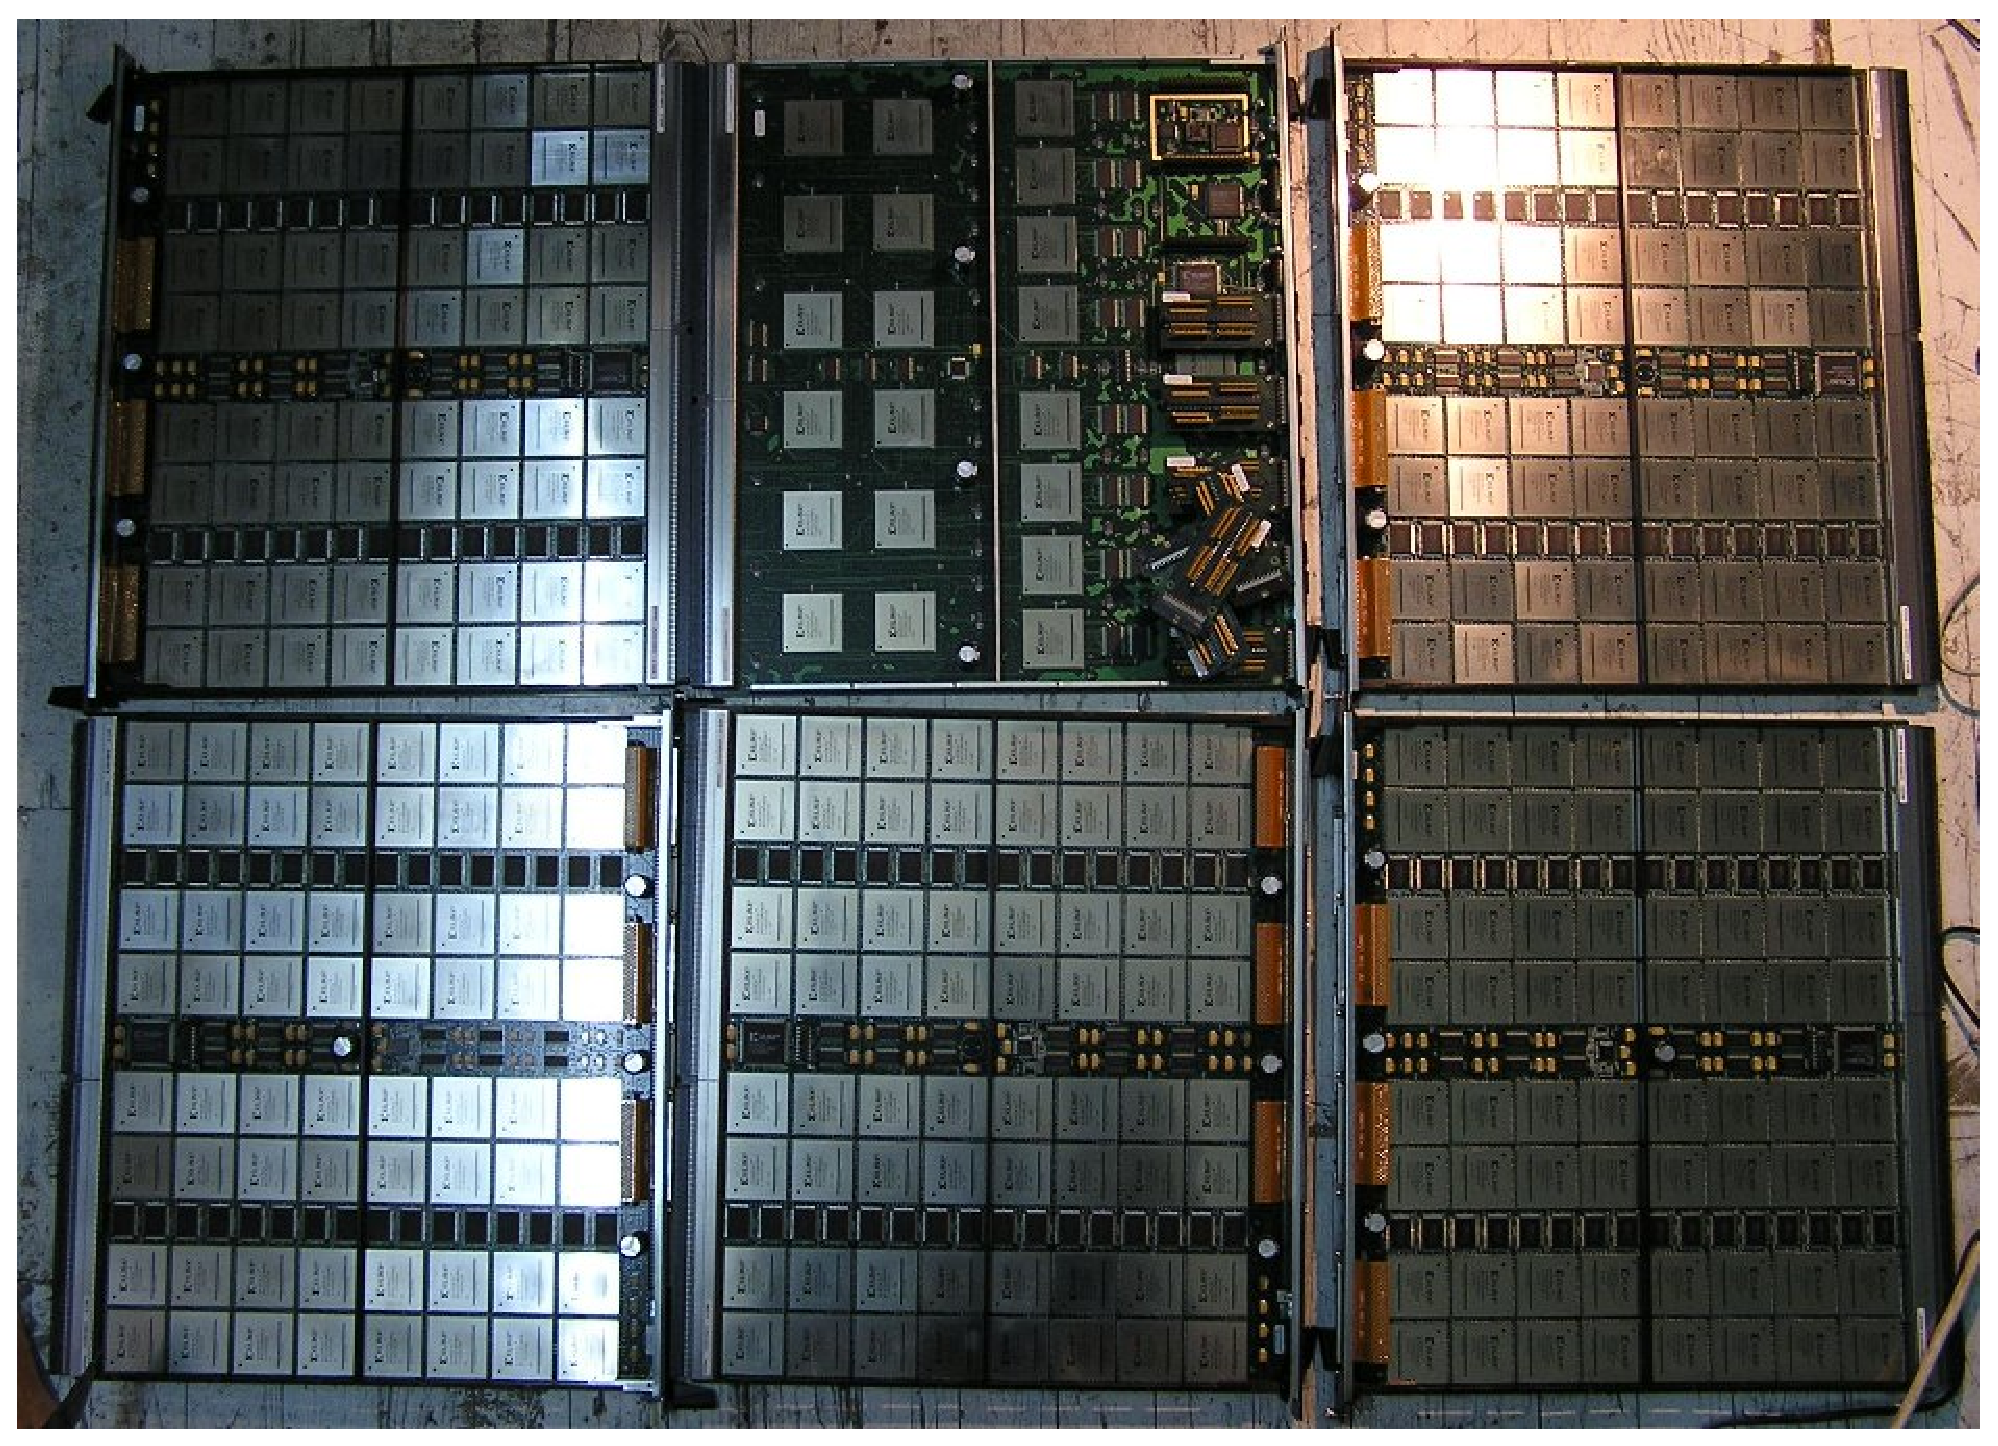
\includegraphics[height=95mm]{ikosboards.eps}
\caption{FPGA boards of the Ikos Pegasus ASIC emulator (ca. 1999)}
\label{fig:ikos}
\end{figure}

But today, the cost of fast high-density FPGAs is falling and these devices are becoming available to the general public. For an example of this trend, I would mention the Ikos Pegasus application specific integrated circuit (ASIC) emulator, whose insides are depicted in figure~\ref{fig:ikos}. The CPU core used in the system-on-chip described in this thesis occupies alone 60\% of the resources of one of the XC4036XL FPGAs of this device, and runs at 30MHz. The Ikos Pegasus was a state-of-the-art device a decade ago. It consumes up to 3 kilowatts of power, weights dozens of kilos and costed the equivalent of several millions of SEK. The same CPU core now occupies about 15\% of a modern FPGA costing less than 500 SEK, where it runs in excess of 100MHz.

This evolution makes it possible to implement complex high-performance system-on-chips (SoC) that can be modified and improved by anyone, thanks to the flexibility of the FPGA platform.

This master thesis introduces Milkymist\texttrademark \cite{Milkymist}, a fast and resource-efficient FPGA-based system-on-chip designed for the application of rendering live video effects during performances such as concerts, clubs or contemporary art installations. Such effects are already popularized by artists known as ``video jockeys'', or ``VJs''.

Besides the fact that this is an interesting, creative and popular application, it is also demanding in terms of computational power and memory performance. It would make Milkymist a proof that high performance open source system-on-chip design is possible in practice; with a view to help, foster and catalyze similar ``open hardware'' initiatives. As the Milkymist system-on-chip is entirely made of synthesizable Verilog and, for the most part, released under the GNU GPL, its code can be re-used by other open hardware projects.

Meeting the performance constraints while still using cheap and relatively small FPGAs is perhaps the most interesting and challenging technical point of this project, and it could not be done without considerable work in the field of computer architecture. This is what this master thesis covers.

\section{Background}
\subsection{Video synthesis}
MilkDrop~\cite{milkdrop} is a popular open source video synthesis framework that was originally made to develop visualization plugins for the Winamp audio player. People have since then ported MilkDrop to many different platforms and made it react to live events, such as captured audio or movements of a WiiMote remote control.

The idea behind the Milkymist project is to implement an embedded video synthesis platform on a custom open source system-on-chip that is based on the same rendering principle of MilkDrop, but with more control interfaces and features.

\begin{figure}[htp]
\centering
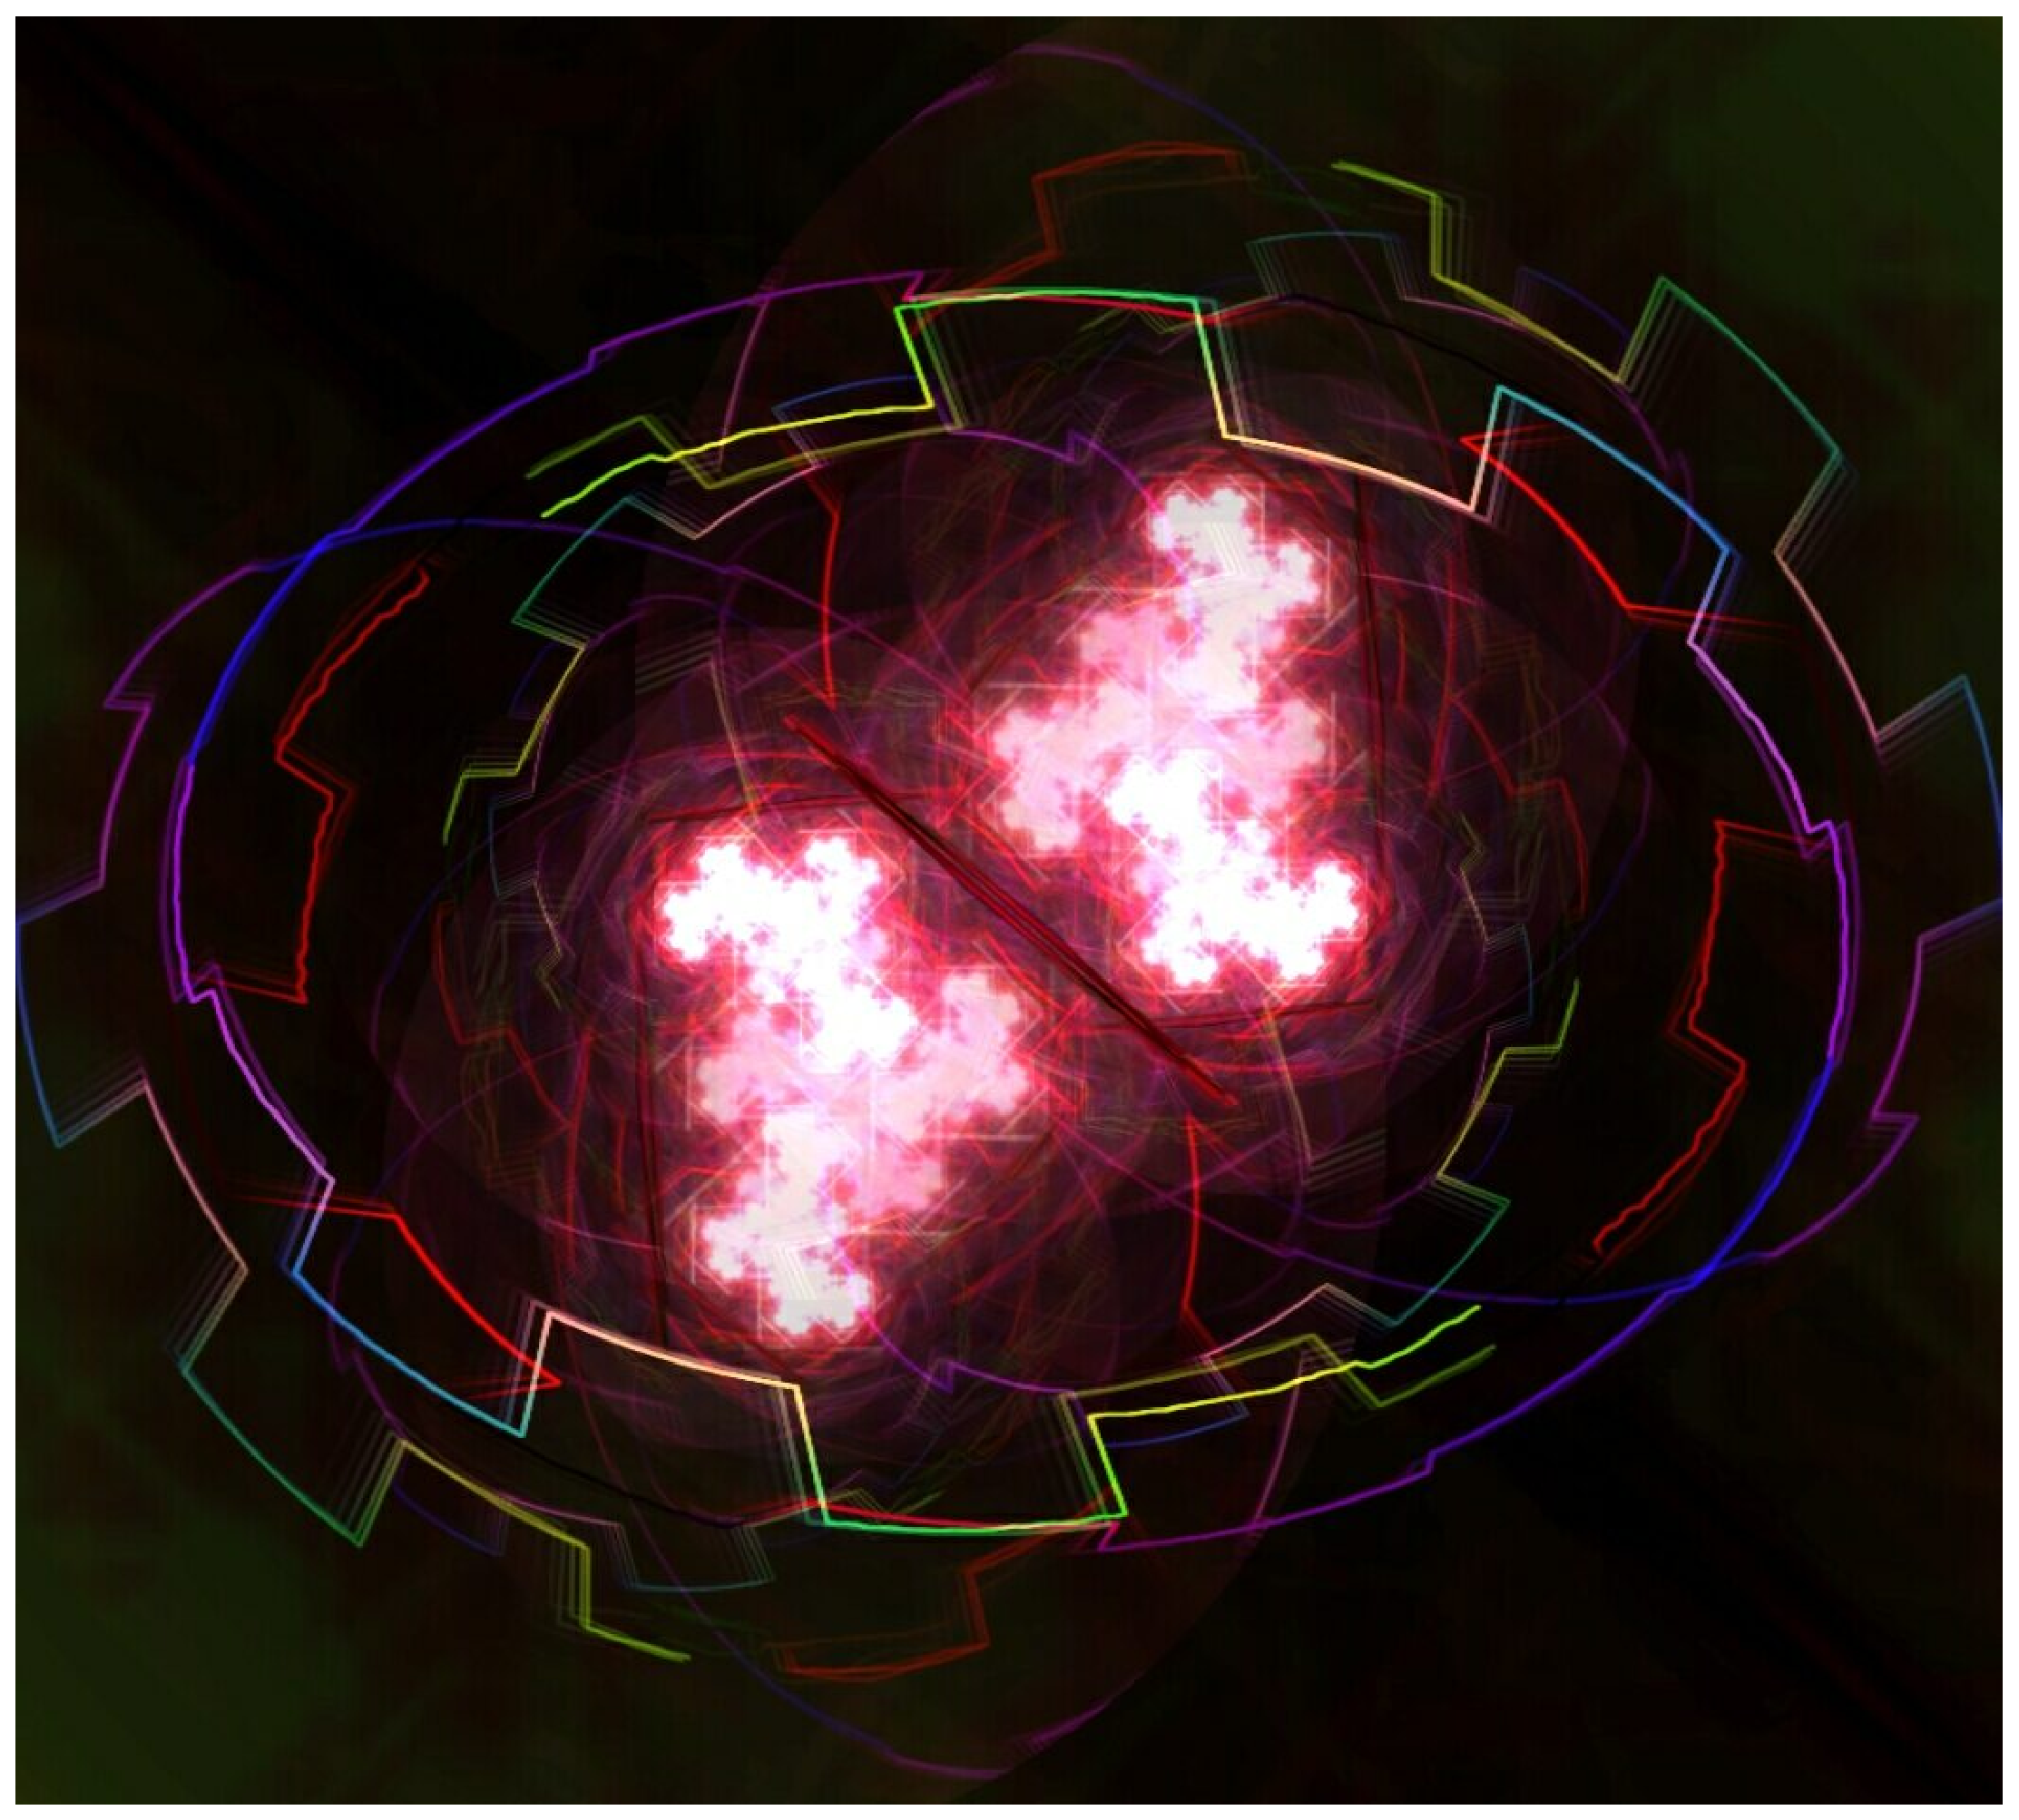
\includegraphics[height=65mm]{milkdrop2.eps}
\caption{Sample video frame from the MilkDrop visual synthesizer.}
\label{fig:milkdrop}
\end{figure}

\subsection{Open source SoC platforms}
There is an existing effort to build open source system-on-chips. It is interesting to review these projects in order to look forward to building upon them -- possibly adding hardware accelerators or performing other modifications in order to improve performance.

There are many SoC designs available on the Internet, which are more or less mature. The system-on-chip projects listed here meet the following criteria:
\begin{itemize}
\item they have been shown to work on at least one FPGA board
\item they are released under an open source license
\item they comprise a synthesizable RISC CPU
\item the CPU is supported by a C and C++ compiler
\item they include a RS232 compatible UART (for a debug console)
\item they support interfacing to off-chip SDRAM memory
\end{itemize}

\subsubsection{OpenSPARC}
OpenSPARC~\cite{opensparc} is the well-known SPARC processor of Sun Microsystems which is now released under an open source license and included into a SoC FPGA project.

Implemented on a FPGA, this processor is extremely resource-intensive. A cut-down version of the CPU core only, called the ``Simply RISC S1'', occupies at least 37000 FPGA look-up tables (LUT) without the caches~\cite{simplyrisc}. This is about twice the logic capacity of the Virtex-4 XC4VLX25 FPGA.

As it turns out, the OpenSPARC architecture is a very complex design which implements a huge number of techniques which increase the software execution speed (instructions per clock cycle). While this is a wise choice for a software-centric processor implemented on a fully custom semiconductor chip, with a FPGA process it is more appealing to keep the software processor simple in order to save resources and make room for custom hardware accelerators, taking advantage of the FPGA flexibility.

\subsubsection{GRLIB}
GRLIB~\cite{grlib} is a very professional and standard-compliant library of SoC cores. The library features a comprehensive set of cores: AMBA AHB/APB bus control elements, the LEON3 SPARC processor, a 32-bit PC133 SDRAM controller, a 32-bit PCI bridge with DMA, a 10/100/1000 Mbit Ethernet MAC,  16/32/64-bit DDR SDRAM/DDR2 SDRAM controllers and more.

However, its drawbacks are:
\begin{itemize}
\item Code complexity. GRLIB is written in VHDL and makes intensive use of custom types, packages, generate statements, etc.
\item Cores are not self-contained. GRLIB defines many ``building blocks'' that are used everywhere else in the code, making it difficult to re-use code in another project which is not based on GRLIB.
\item Significant FPGA resource usage. Synthesized with Xilinx ISE 11.3, a system comprising the LEON3 SPARC processor with a 2-way set-associative 16kB cache and no memory management unit (MMU), the DDR SDRAM controller, a RS232 serial port, and a Ethernet 10/100 MAC uses 13264 FPGA look-up tables (LUT). They map to 79\% of the Virtex-4 XC4VLX25 FPGA. This undermines the possibility of adding hardware acceleration cores.
\item Relatively low clock frequency. With the same parameters as above, the maximum clock frequency is 84MHz.
\end{itemize}

Because of these reasons, GRLIB was not retained.

\subsubsection{ORPSoC (OpenRISC)}
ORPSoC is based on the OpenRISC~\cite{openrisc} processor core, which is the flagship product of OpenCores, a community of developers of open source system-on-chips. ORPSoC is essentially maintained by ORSoC AB.

ORPSoC notably features the OpenRISC OR1200 processor core, the Wishbone~\cite{wishbone} bus, comprehensive debugging facilities, a 16550-compatible RS232 UART, a 10/100Mbps Ethernet MAC and a SDRAM controller.

Unfortunately, ORPSoC is resource-inefficient and extremely slow, mainly because of the OpenRISC implementation which is not optimized for synthesis and the poorly designed SDRAM controller. Using ORSoC AB's reference design, a C program takes more than a dozen of seconds to copy a 16MB SDRAM buffer from one memory location to another.

OpenRISC and ORPSoC therefore do not seem to be a good platform for the performance-demanding video synthesis application.

\subsubsection{LatticeMico32 System}
This product~\cite{mico32} from the FPGA vendor Lattice Semiconductor is comparable to Microblaze~\cite{microblaze} and Nios II~\cite{nios} from its competitors, respectively Xilinx and Altera.

Like its competing products, LatticeMico32 System features a broad library of light, fast and FPGA-optimized SoC cores.

One interesting move made by Lattice Semiconductor is that parts of the LatticeMico32 System are released under an open source license, and most notably the custom LatticeMico32 microprocessor core. LatticeMico32 System is also based upon the Wishbone~\cite{wishbone} bus, whose specification is free of charge and freely distributable.

While it is perhaps technically possible to build Milkymist on top of the LatticeMico32 System, there are licensing issues concerning most notably the DDR SDRAM controller which is proprietary.

However, the LatticeMico32 microprocessor core is interesting. Synthesized for the XC4VLX25 with the 2-way set-associative caches enabled, it occupies only about 2400 LUTs and runs at more than 100MHz.

\section{Problem statement}
According to this background, for the video synthesis application it seems relevant to:

\begin{itemize}
\item develop a fast, resource-efficient and FPGA-optimized system-on-chip
\item develop an efficient memory subsystem
\item use a light-weight softcore CPU
\item develop custom hardware accelerators
\end{itemize}

This thesis focuses on the computer architecture problems and concepts behind these points.

\chapter{Memory subsystem}
\section{Attacking the memory wall}
\label{sec:memorywall}
A recurrent point in many modern computer systems is the memory performance problem. The term \textit{memory wall} was coined~\cite{memorywall} to refer to the growing disparity of performance between logic such as CPUs and off-chip memories. While microprocessor performance has been improving at a rate of 60 percent per year, the access time to DRAM has been improving at less than 10 percent per year~\cite{memvscpu}.

Memory performance is measured with two metrics:
\begin{itemize}
\item \textit{bandwidth}, which is the amount of data that the memory system can transfer during a given period of time.
\item \textit{latency}, which is the amount of time that the memory system spends between the issue of a memory read or write request and its completion.
\end{itemize}

A memory system can have both high bandwidth and latency. If the logic making the memory accesses is able to issue requests in a pipelined fashion, sending a new request without waiting for the previous one to complete, high latency will not have an impact on bandwidth.

Latency and bandwidth are however linked in practice. Decreasing the latency also increases the bandwidth in many cases, because latency blocks sequential processes and prevents them from utilizing the full available bandwidth.

High-end processors for servers and workstations have a good ability to cope with relatively high memory latency, because techniques such as out-of-order execution and hardware multi-threading enable the processor to issue new instructions even though one is blocking on a memory access.

Thus, most of today's SDRAM controllers do a lot to optimize bandwidth but have little focus on latency. Bandwidth-optimizing techniques include:
\begin{itemize}
\item reordering memory transactions to maximize the page mode hit rate.
\item grouping reads and writes together to reduce write recovery times. Along with the above technique, this has a detrimental impact on latency because of the delays incurred by the additional logic in the address datapath.
\item running the system and the SDRAM in asynchronous clock domains in order to be able to run the SDRAM at its maximum allowable clock frequency. This requires the use of synchronizers or FIFOs, which have a high latency.
\item configuring the SDRAM at high CAS latencies in order to increase its maximum allowable clock frequency. This trend is best illustrated by the advent of DDR2 and DDR3 memories whose key innovation is to run their internal DRAM core at a submultiple of the I/O frequency with a wide data bus which is then serialized on the I/O pins. Since the internal DRAM core has a latency comparable to that of the earlier SDR and DDR technologies, the number of CAS latency cycles relative to the I/O clock is also multiplied.
\end{itemize}

An extreme example of these memory controller bandwidth optimizations is the MemMax\textregistered ~DRAM scheduler~\cite{memmax}. This unit sits on top of an already existing memory controller (which already has its own latency), adding seven stages of complex and high-latency pipelining that produces a good - but compute-intensive - DRAM schedule. The actual efficiency of this system has been questioned~\cite{dramqos} because of that significant increase in latency.

\section{Another approach}
The out-of-order execution and hardware multithreading processor optimizations discussed above that cope with high memory latency are complex and impractical in the context of small and cheap embedded systems, especially those targetted at FPGA implementations. For example, FPGA implementations of the OpenSPARC~\cite{opensparc} processor, which employs such optimizations, typically require an expensive high-end Xilinx XUPV5 board whose Virtex-5 FPGA alone costs roughly 13000 SEK.

Milkymist therefore uses simple in-order execution schemes in its CPU and in its accelerators, and strives to improve performance by focusing on reducing the memory latency.

The memory system features that improve latency (but also bandwidth) are discussed below.

\section{Memory system features}
\subsection{Single SDRAM and system clock domain}
The typical operating frequency of early SDR and DDR SDRAM (technologies that are prior to DDR2 and do not have a clock divider for the internal DRAM core) is close to the 100MHz frequency at which the FPGA is able to meet timing for the complete SoC. Thus, it was decided to run the DRAM and the system synchronously in order to remove the need for any clock domain transfer logic and reduce latency. The SDRAM I/O registers are clocked by the system clock, and timing of the SDRAM interface is met through the use of calibrated on-chip delay elements and delay-locked-loops (DLLs) to generate the off-chip SDRAM clock and the data strobes.

\subsection{Page mode control algorithm}
The Milkymist memory controller takes the so-called ``page mode gamble'': after an access, the DRAM row is left open in the hope that the next transaction to the memory bank will occur within the same row. If the memory controller is right, the read of write command can be immediately registered into the SDRAM, and only the CAS or write latency is incurred. If the memory controller is wrong, it must first precharge the DRAM bank and open the correct row, causing extra delays.

Thus, if the memory controller is often wrong, taking the page mode gamble will actually impact performance negatively. However, a study has shown~\cite{pagemode} that, with typical memory timings, the point at which the gamble pays off is for a page hit probability of 0.375 only, attainable with many practical memory access patterns.

Page hit probability is also improved by the ability of the Milkymist memory controller to track open rows independently in each of the four memory banks that commercial SDRAM chips are equipped with.

This optimization positively affects both latency and bandwidth.

\subsection{Burst accesses}
\label{subsec:fmlburst}
All memory accesses are made using bursts, i.e. when an access for a word is made, the following words are also read or written. Burst mode is a feature of the SDRAM chips: only one read of write command is sent to them, and several words are transferred on subsequent clock cycles.

Using bursts frees the bus and DRAM control signals while other words are transferred, allowing the issue of new commands overlapping the data phase of the previous transaction.

Burst access is a form of prefetching that improves latency. It is only efficient when the prefetched data can be used by the requesting bus master. In the Milkymist system-on-chip, this is often the case:
\begin{itemize}
\item The CPU core has a cache which accesses memory by complete cache lines. Thus, if the cache line length is a multiple of the burst length, the bursts can be easily fully memorized.
\item The video framebuffer repeatedly reads the same block of data in a sequential manner, and can easily make full use of the prefetched data assuming that is has sufficient on-chip buffer space.
\item The texture mapping unit also has a cache and a write buffer which work well with burst accesses. This will be discussed in Chapter~\ref{ch:tmu}.
\end{itemize}

\subsection{Burst reordering}
\label{subsec:fmlborder}
This feature enables the use of the critical-word-first scheme in caches, reducing the overall memory latency.

When a request is issued at an address which is not a multiple of the burst length, the order of the words in the burst is changed so that the first word that comes out is the very word that is at the requested memory address. The prefetch address is then incremented and wraps to stay within the same burst.

For example, assuming a burst length of 4:
\begin{itemize}
\item a request at address 0 fetches words 0, 1, 2 and 3 (in this order)
\item a request at address 2 fetches words 2, 3, 0 and 1 (in this order)
\end{itemize}

\subsection{Pipelining}
\label{subsec:fmlpipe}
The memory bus of Milkymist~\cite{fml} is pipelined. During the transfer of the prefetched (burst) data, a new request can be issued. This is illustrated for a read request by the table below:

\begin{tabular}{|c|c|c|c|c|c|c|c|}
\hline
\textbf{Address} & A1 & A1 & A1 & A2 & A2 & A2 & A2 \\
\hline
\textbf{Data} & -- & -- & M(A1) & M(A1+1) & M(A1+2) & M(A1+3) & M(A2) \\
\hline
\end{tabular}\\

\begin{tabular}{|c|c|c|c|}
\hline
\textbf{Address (cont.)} & -- & -- & --\\
\hline
\textbf{Data (cont.)} & M(A2+1) & M(A2+2) & M(A2+3) \\
\hline
\end{tabular}

Together with burst access, this helps acheiving high performance: the memory controller can hide DRAM latencies and row switch delays by issuing the requests to the DRAM in advance, while the previous transaction is still transferring data.

\section{Practical implementation}
The Milkymist SoC uses 32-bit DDR SDRAM, configured to its maximum burst length of 8. Since the DDR SDRAM transfers two words per clock cycles (one on each edge), this is turned by the I/O registers into bursts of four 64-bit words synchronous to the system clock.

\begin{table}
\centering
\begin{tabular}{|l|l|}
\hline
\textbf{Task} & \textbf{Required bandwidth} \\
\hline
VGA framebuffer, 1024x768, 75Hz, 16bpp & 950Mbps \\
\hline
Texture mapping, 1024x768, 30fps, 16bpp & 750Mbps \\
\hline
NTSC input, 720x576, 30fps, 16bpp & 200Mbps \\
\hline
Software and misc. & 300Mbps \\
\hline
\textbf{Total} & \textbf{2.2Gbps} \\
\hline
\end{tabular}
\label{tab:membw}
\caption{Estimate of the memory bandwidth consumption}
\end{table}

The memory is run at 100MHz, yielding a peak theoretical bandwidth of 6.4Gbps, which is more than enough for the intended video synthesis application (Table~\ref{tab:membw}). This bandwidth is however never attained: events such as switching DRAM rows which takes significant time and, to a lesser extent, DRAM refreshes introduce dead times on the data bus. Furthermore, a bandwidth margin is kept to enable potential future extensions such as the support of 24bpp or 32bpp color depths, which would increase bandwidth consumption.

\begin{figure}[H]
\centering
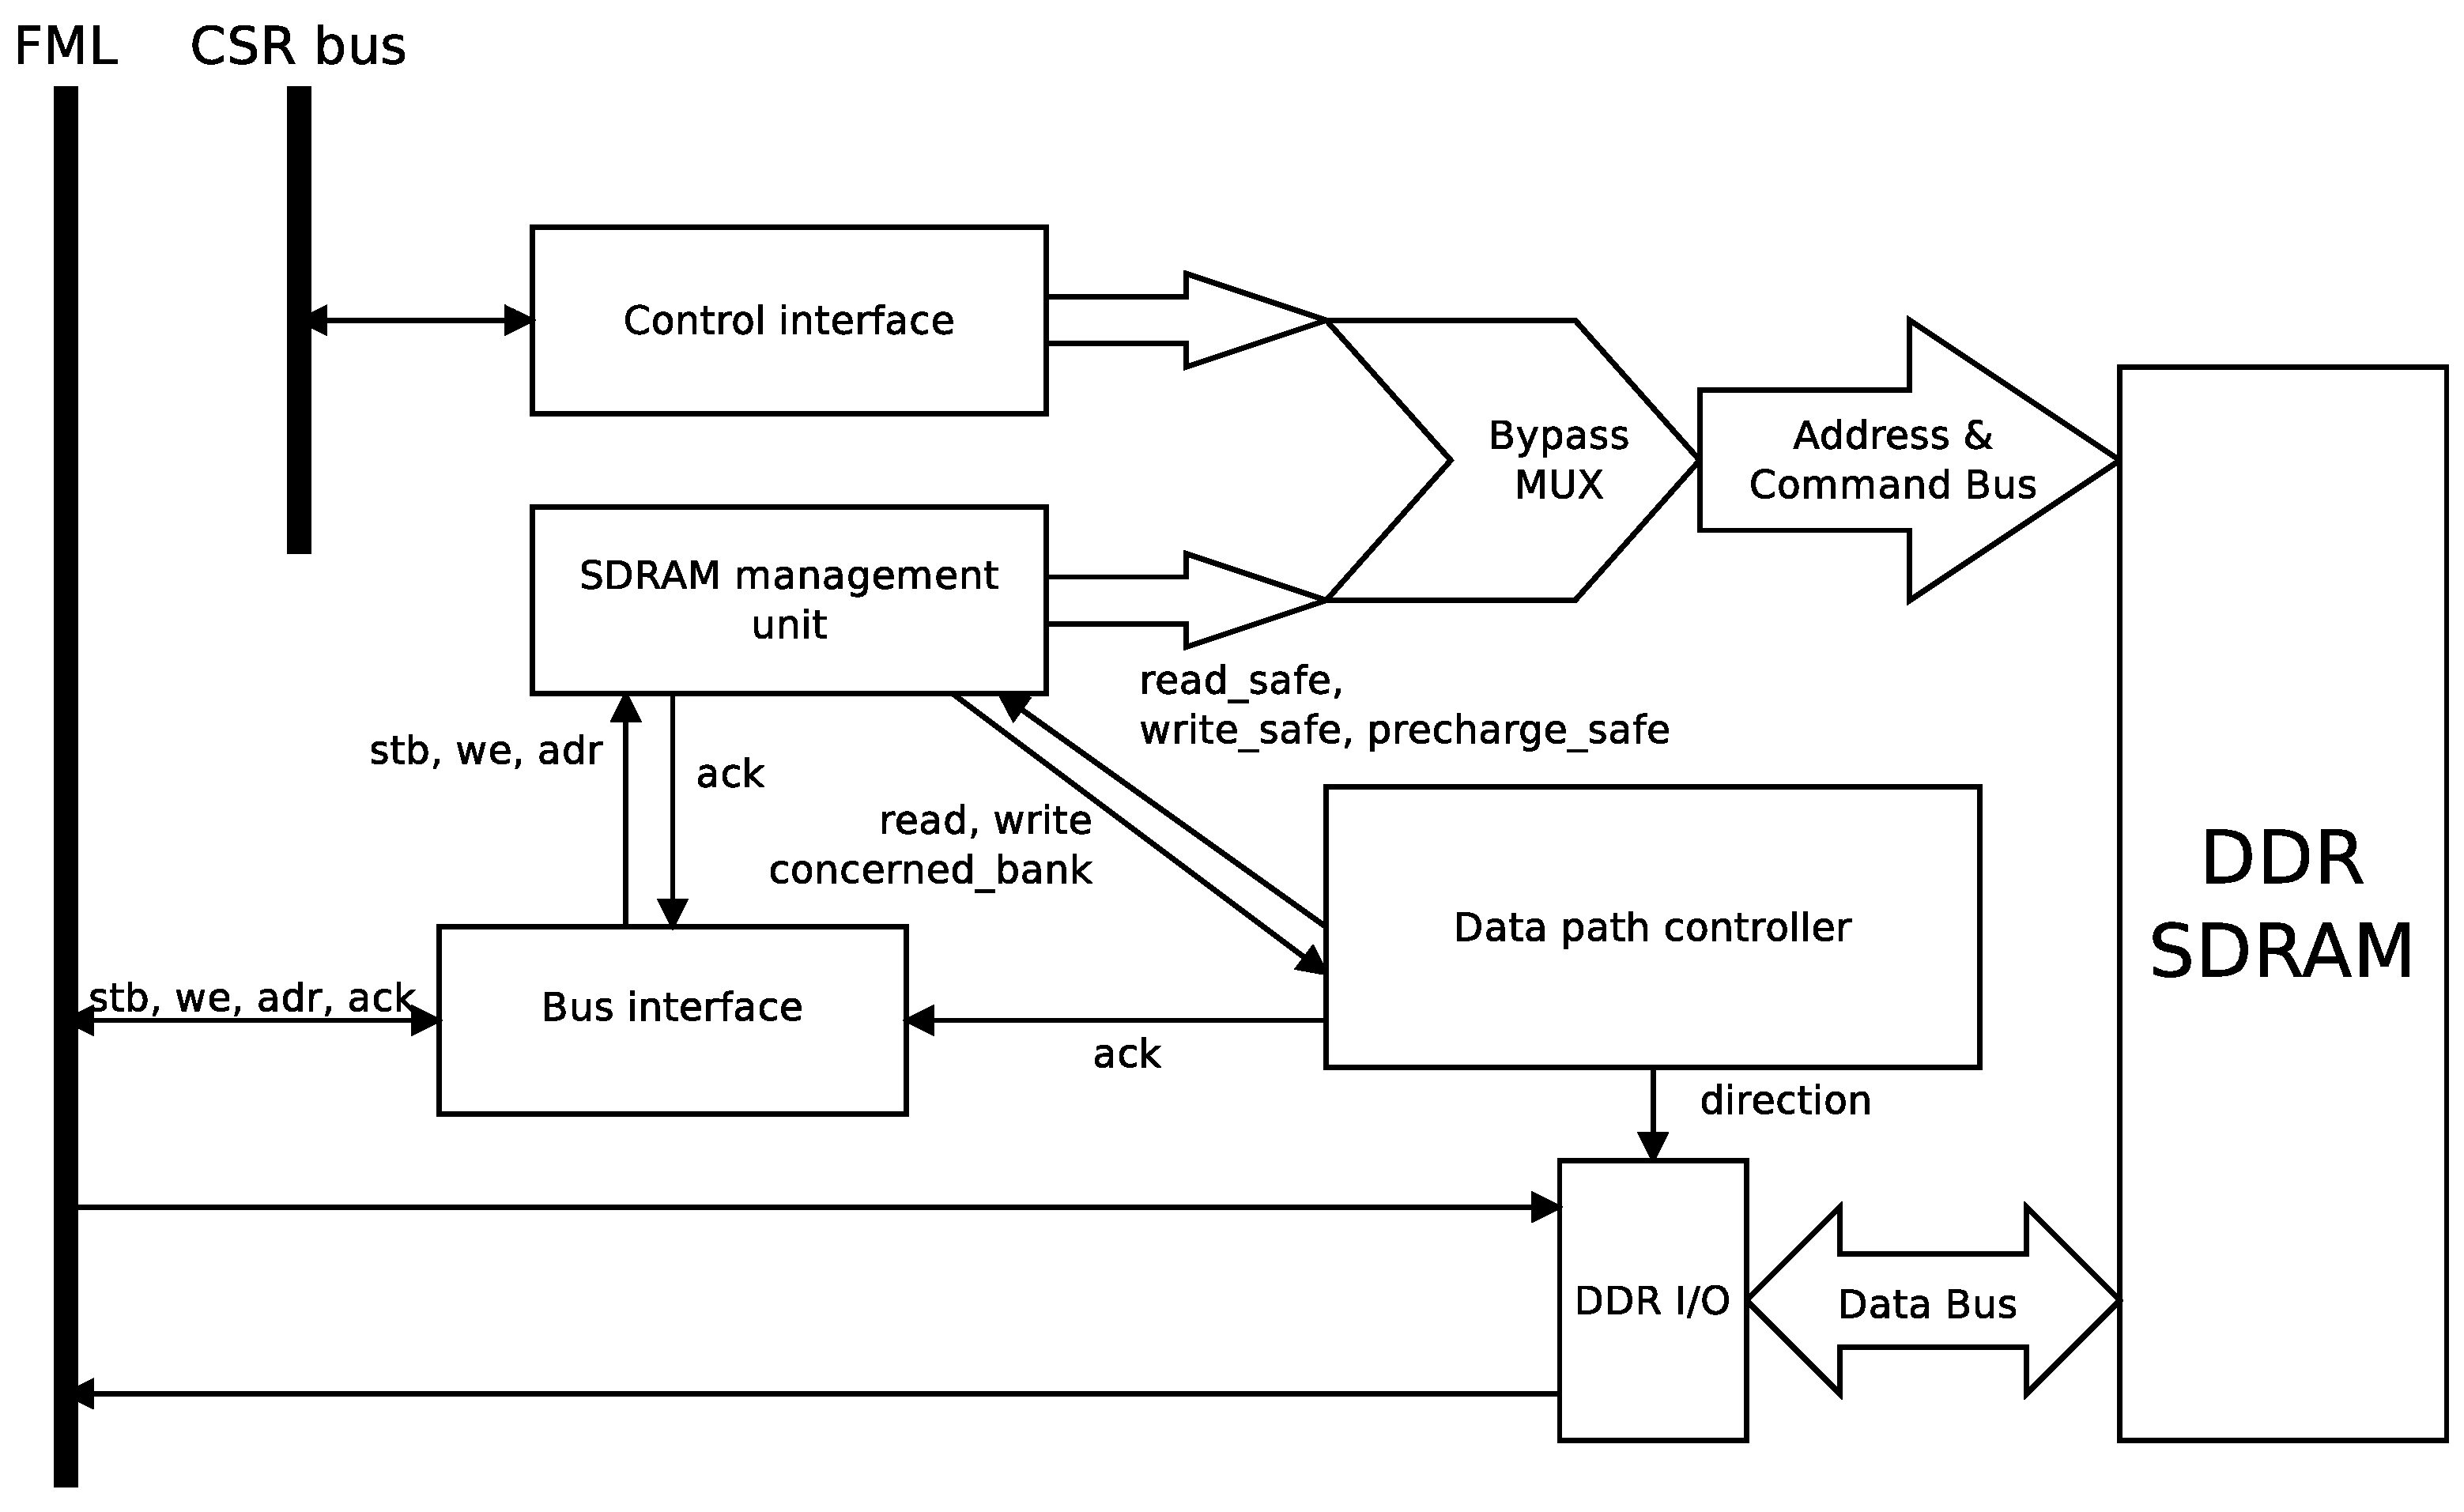
\includegraphics[height=85mm]{hpdmc_block.eps}
\caption{Block diagram of the HPDMC architecture.}\label{fig:hpdmc_block}
\end{figure}

The architecture of the memory controller, dubbed HPDMC (for ``High Performance Dynamic Memory Controller''), is outlined in figure~\ref{fig:hpdmc_block}.

The control interface is used by the system to configure the controller, and also to issue the start-up sequence to the SDRAM. Indeed, SDRAM chips require a sophisticated sequence of commands upon power-up. In many memory controller designs, a hardware finite state machine is used to issue this command sequence. In order to save hardware resources, the system used  here leaves this task to the software, and, for this purpose, includes a ``bypass MUX'' that routes directly a configuration and status register of HPDMC to the SDRAM command and address pins. Once the SoC has run a software routine that sends the correct initialization sequence to the SDRAM, it switches permanently the bypass MUX to the ``SDRAM management unit'' and can use off-chip memory normally.

The SDRAM management unit is a finite state machine that translates the two high-level memory commands ``read burst at address'' and ``write burst at address'' into a series of lower-level commands understandable by the SDRAM chips (precharge bank, select row, read from row, etc.). The management unit is responsible for keeping track of the open rows, detecting page hits, switching rows, and issuing periodic DRAM refresh cycles.

The management unit is connected to the ``data path controller'', that follows the activities performed by the management unit in order to decide the direction of the bidirectional I/O pins (they should be set as outputs for writes and as input for reads). The data path controller is also responsible for sending signals to the management unit that indicate if it is safe to perform certain low-level operations. For example, the \verb!read_safe! signal goes low immediately after a read command is issued, because if another one were sent immediately after, the two resulting bursts would overlap in time and this could not work because there is only one set of data pins. Eventually, the data path controller takes into account the SDRAM write and read latencies to generate an acknowledgement signal when the data is actually there (or needs to be sent to the SDRAM) after a ``read row'' or ``write row'' command has been sent to the SDRAM.

Finally, the bus interface is a piece of glue logic that connects the SoC pipelined memory bus (FML) to the data path controller and the management unit.

HPDMC has been implemented in Verilog HDL, tested and debugged in RTL simulation using a DDR SDRAM Verilog model from Micron, integrated into the SoC, synthesized into FPGA technology, and eventually calibrated and tested by software routines running on the actual hardware.

This design of memory controller, specifically crafted for the Milkymist project and released under the GNU GPL license on the internet, has been picked up by the NASA for a software defined radio project and may be put up onboard the international space station in 2011. Gregory Taylor, Electronics Engineer at the NASA Jet Propulsion Laboratory, writes:

\textit{While searching for a suitable SDRAM controller for the Jet Propulsion Laboratory's Software-Defined Radio onboard NASA's CoNNeCT experiment, I found S\'ebastien's HPDMC SDRAM controller on OpenCores.org. We needed a controller that was both high performance and well documented. Though the original HPDMC controller was designed for DDR SDRAM with a 32-bit bus, S\'ebastien clearly explained the modifications necessary to adapt the controller to our Single Data Rate, 40-bit wide SDRAM chip. I found the code to be well documented and easy to follow. The performance has met our requirements and the FPGA size requirement is small.}

\textit{The Communication Navigation and Networking Reconfigurable Testbed (CoNNeCT) experiment to be installed onboard the ISS is designed for the next generation of SDRs conforming to the Space Telecommunications Radio Systems (STRS) open architecture standard. The HPDMC controller will likely find its way into one or more loadable waveform payloads in the JPL SDR, and perhaps be used in other NASA projects as well. It may eventually find its way into deep space.}

\section{Performance measurement}
\subsection{Introduction}
We wanted to validate and characterize the memory system performance (actual latency and bandwidth) and get an upper bound of of its ability to sustain loads, by extrapolating the maximum bandwidth one could get assuming the memory access time remains constant.

Since the memory performance depends on the particular access pattern that the system makes (because of the controller taking the page mode gamble, we wanted to take the measurements on the real system while it is rendering video effects in order to get an accurate result.

\subsection{Method}
A logic core has been added to the SoC that snoops on the memory bus activity in order to report the average latency and bandwidth.

That logic core exploits properties of the FastMemoryLink signaling in order to reduce its complexity to two counters that measure, for a given time period, the number of cycles during which the strobe and acknowledgement signals are active. Several parameters can then be computed:
\begin{itemize}
\item the \textbf{net bandwidth} carried by the link (based on the amount of data that the link has actually transferred)
\item the \textbf{average memory access time}, which is the time, in cycles, between the request being made to the memory controller and the first word of data being transferred.
\item the \textbf{bus occupancy} which is the percentage of time during which the link was busy and therefore unavailable for a new request.
\end{itemize}

\subsection{Results}
Results are summarized in table~\ref{tab:memperformance}. The first line corresponds to a system running the demonstration firmware with the video output enabled at the standard VGA mode of 640x480 at 60Hz (therefore continuously scanning the screen with data from system memory), but not rendering a preset. The other lines represent the results while the demonstration firmware is rendering different MilkDrop presets, still at the same video resolution.

\begin{table}
\centering
\begin{tabular}{|l|l|l|l|l|}
\hline
\textbf{Preset} & \textbf{Bandwidth} & \textbf{Occupancy} & \textbf{AMAT} & \textbf{Bandwidth bound}  \\
\hline
Idle & 293 Mbps & 7 \% & 5.52 &  Mbps \\
\hline
Geiss - Bright Fiber Matrix 1 & 1067 Mbps & 31 \% & 6.58 &  Mbps \\
\hline
Geiss - Swirlie 3 & 1160 Mbps & 34 \% & 6.71 &  Mbps \\
\hline
StudioMusic - Twisted Galaxy & 942 Mbps & 25 \% & 5.94 & Mbps \\
\hline
Geiss - Spacedust & 1024 Mbps & 30 \% & 6.67 &  Mbps \\
\hline
Geiss - Anomaly 2 & 1127 Mbps & 33 \% & 6.58 &  Mbps \\
\hline
Aderrasi - Candy Avian & 923 Mbps & 27 \% & 6.52 &  Mbps \\
\hline
\end{tabular}
\caption{Memory performance in different conditions (Milkymist 0.5).} \label{tab:memperformance}
\end{table}

\chapter{SoC interconnect}
The general SoC block diagram and its interconnect is outlined in~\ref{fig:block}. Not all the blocks are ready at the time of this writing, nor all of them are within the scope of this Master's thesis!

More specifically, the following components are not developed yet:
\begin{itemize}
\item Ethernet controller
\item microSD controller (the current prototype use a CF card through Xilinx SystemACE)
\item USB controller
\item Video input
\item IR receiver
\item MIDI controller
\item DMX512 controller
\end{itemize}

This chapter explains how the different interconnect busses work, what their features are, why they are there, and how they are communicate with each other.

\begin{figure}
\centering
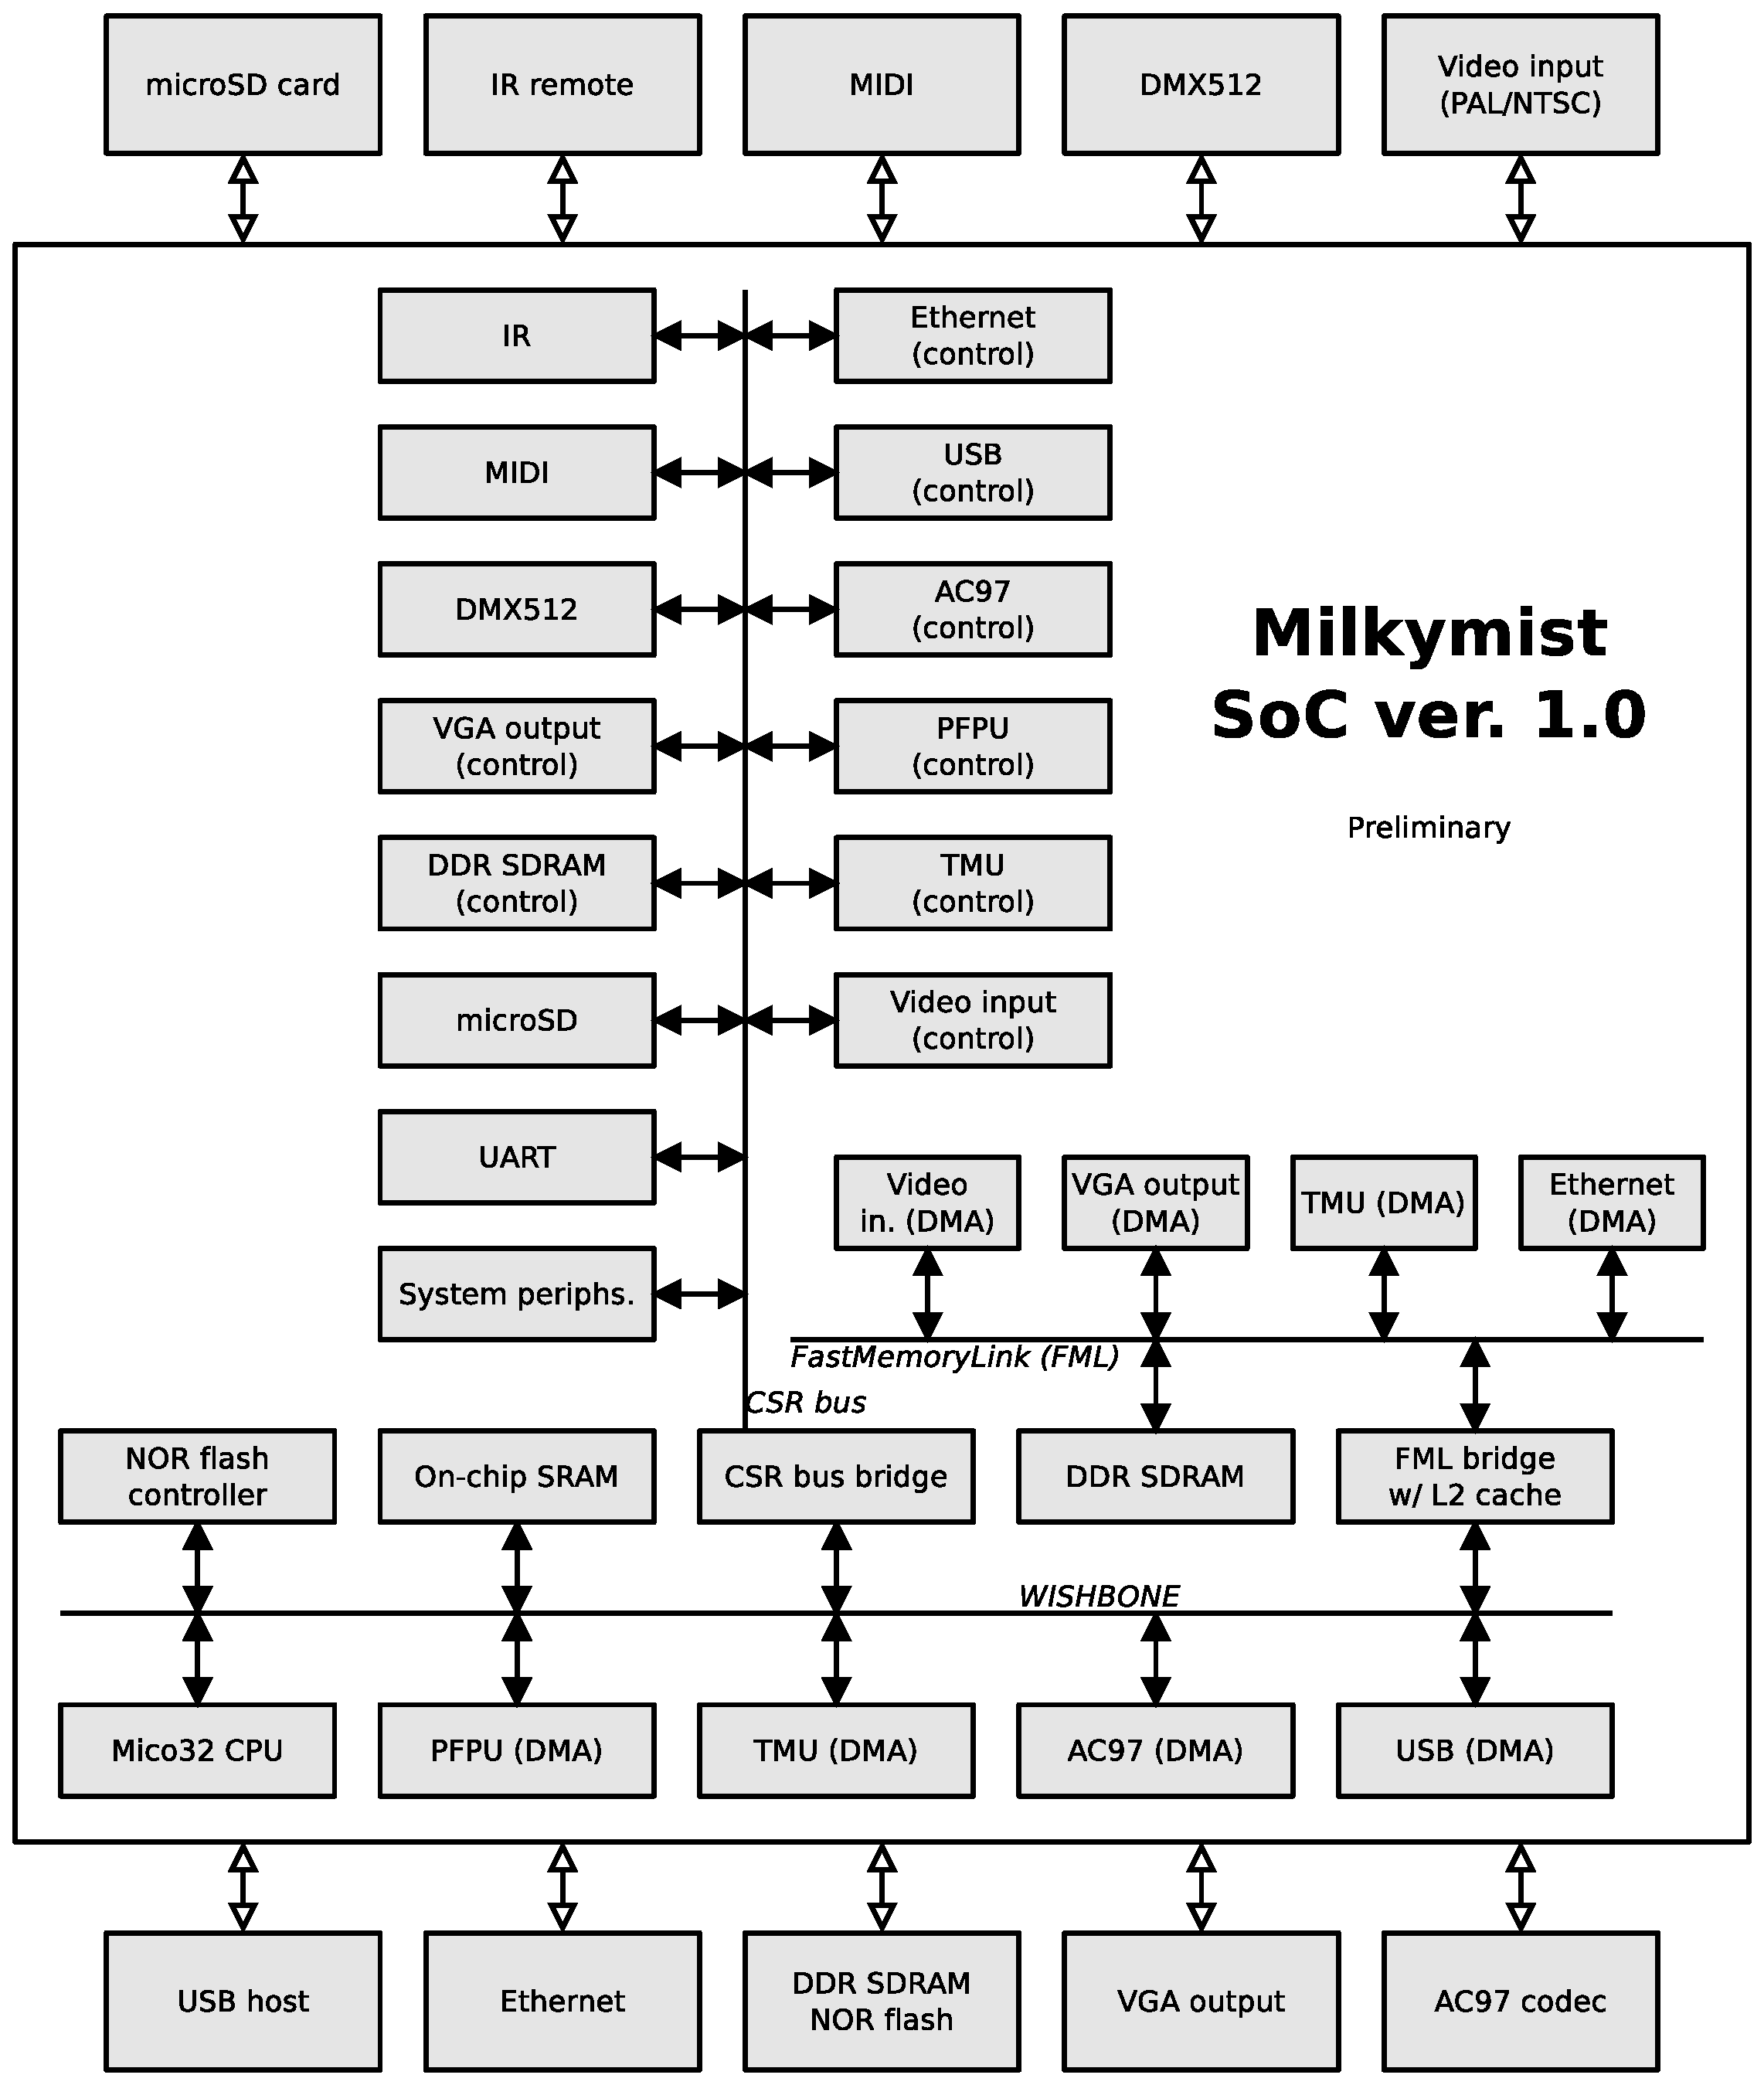
\includegraphics[height=170mm]{soc_architecture.eps}
\caption{SoC block diagram}
\label{fig:block}
\end{figure}

\section{General SoC interconnect: the Wishbone bus}
Wishbone~\cite{wishbone} is a general purpose royalty-free SoC bus with open specifications, advocated by the maintainers of the OpenCores.org website.

Wishbone is a synchronous sequential bus with support for variable latency (wait states) through the use of an acknowledgement signal that marks the end of the transaction. Burst modes (automatic transfer of consecutive words) are supported and are configurable on a per-transaction basis (i.e. bursts of arbitrary lengths and single-word transactions can be freely mixed on the same bus). However, there is no pipelining.

Wishbone is used around the SoC's LatticeMico32 CPU core and for simple DMA masters which have modest requirements of bandwidth and of volume of transferred data. As will be explained in Section~\ref{sec:fmlbrg}, connecting DMA masters that transfer small amounts of data (which can fit in the L2 cache) to the same bus as the CPU simplifies dealing with cache coherency issues.

The data width used for the Wishbone bus is 32, yielding a peak bandwidth of 3.2Gbps when the system is running at 100MHz.

\section{Configuration and Status Registers: the CSR bus}
Milkymist uses memory-mapped I/O through configuration and status registers.

If these registers were directly accessed by the Wishbone CPU bus, two problems would arise:
\begin{itemize}
\item Connecting all peripherals on the same Wishbone bus involves large multiplexers and high fanout signals, posing routing and timing problems.
\item Wishbone requires the generation of an acknowledgement signal by each slave core. This signal is useful in many cases, as it supports peripherals with a variable latency. However, configuration and status register files are usually implemented with actual registers (flip flops) or SRAM, which can always be accessed in one clock cycle. Thus, there is no need for variable latency and the acknowledgement signal. Keeping this signal for the configuration and status registers wastes hardware resources and development time.
\end{itemize}

To alleviate these problems, the CSR bus has been developed~\cite{csr} and used in the system through a bus bridge.

The CSR bus is a simpler bus than Wishbone, where all transfers are done in one cycle. It has an interface similar to that of synchronous SRAM, consisting only of address, data in, data out and write enable pins and clocked by the system clock.

A bridge connects the CSR bus to the CPU Wishbone bus, to allow transparent memory-mapped access to the configuration and status registers by the software. This bridge includes registers for all the signals crossing the two busses, relaxing the timing constraints.

\section{High-throughput memory access bus: the FML bus}
FastMemoryLink (FML)~\cite{fml} was co-designed with HPDMC (the memory controller) as a on-chip bus tailored to access SDRAM memories at high speed while keeping the memory controller simple. Its key features are listed below.

\subsection{Variable latency}
SDRAM latency varies a lot depending on the state of the SDRAM at the time the request is issued on the bus. It depends on whether the SDRAM was in the middle of a refresh cycle, whether the bank needs to be precharged, and whether a new row needs to be activated. Therefore, FML provides support for a variable number of wait states, defined by the memory controller, through the use of an acknowledgement signal similar to that of Wishbone.

\subsection{Burst only}
SDRAM is best accessed in burst mode (see Subsection~\ref{subsec:fmlburst}).

However, enabling or configuring burst mode is a relatively lengthy and complex operation, requiring a reload of the SDRAM mode register which takes several cycles. Furthermode, supporting multiple burst lengths makes the scheduling of the transfers more complex to avoid ``overlapping'' transfers that would create conflicts at the data pins.

Therefore, in order to greatly simplify the memory controller, all transfers on FML are made using a fixed and pre-defined burst length.

\subsection{Burst reordering}
This was discussed in Subsection~\ref{subsec:fmlborder}.

\subsection{Pipelining}
The benefits of this feature have already been discussed in Subsection~\ref{subsec:fmlpipe}.

Pipelined requests may come from the same core that issued the initial transfer, or from another core. The FML arbiter would then pipeline the request coming from the other core.

\subsection{Usage}
The data width used for the FML bus is 64, yielding a peak bandwidth of 6.4Gbps when the system is running at 100MHz. This is twice the peak bandwidth of the Wishbone bus. Furthermore, this bus provides a short path to the memory controller, reducing latency and therefore potentially further increasing effective bandwidth, as discussed in Section~\ref{sec:memorywall}.

Peripherals directly connected to FML are typically those which transfer large amounts of data (that would exceed the capacity of the L2 cache presented in Section~\ref{sec:fmlbrg}) and which have high bandwidth requirements (and therefore can take advantage of the bandwidth and latency improvement compared to Wishbone).

In the Milkymist SoC, they are comprised of:
\begin{itemize}
\item the VGA output controller, which needs to continously scan a framebuffer up to several megabytes in size to generate the video signal.
\item the (planned) video input, which writes, every second, dozens of digitized video frames weighting hundreds of kilobytes each.
\item the texture mapping unit (Chapter~\ref{ch:tmu}), which needs to deal with large textures at high speed.
\end{itemize}

\section{Bridging Wishbone to FML}
\label{sec:fmlbrg}
For Wishbone masters (like the CPU) to access SDRAM transparently, it is necessary to bridge the FML bus to the Wishbone bus.

FML is a burst-only bus with a fixed burst length, while with Wishbone, bursts are optional and configured on a per-transaction basis. To be efficient, the bridge must therefore be able to store data and slice it to meet the transfer size requirements of the Wishbone and FML transactions.

A traditional write-back cache with a line length equal to the FML burst length provides an elegant solution to this problem. This cache is referred to as the ``L2 cache'', because, from the CPU point of view, it provides a second level of cache relative to its integrated instruction and data caches.

The bridge provides very limited support for cache coherency. Cache coherency issues arise because of the masters directly connected to the FML bus:
\begin{itemize}
\item The CPU may read a cached copy of a data that has been modified by a FML master.
\item A FML master may read a value that has been modified by the CPU in the cache (dirty line) but not flushed to the SDRAM.
\item A FML master may update a value in SDRAM but not in the cache. The line may then go dirty, and, when flushed, will erase the value written by the FML master.
\end{itemize}

\chapter{Software execution environment}
\section{LatticeMico32}
The heart of the software execution capabilities of the SoC is the LatticeMico32 microprocessor core~\cite{mico32}. It is a classic 6-stage in-order pipelined RISC processor (figure~\ref{fig:lm32arch}) with a custom instruction set supported by the GNU (GCC-based) compiler toolchain. It supports separate instruction and data caches with up to two ways. There are an optional barrel shifter, pipelined multiplier and multi-cycle divider.

\begin{figure}[htp]
\centering
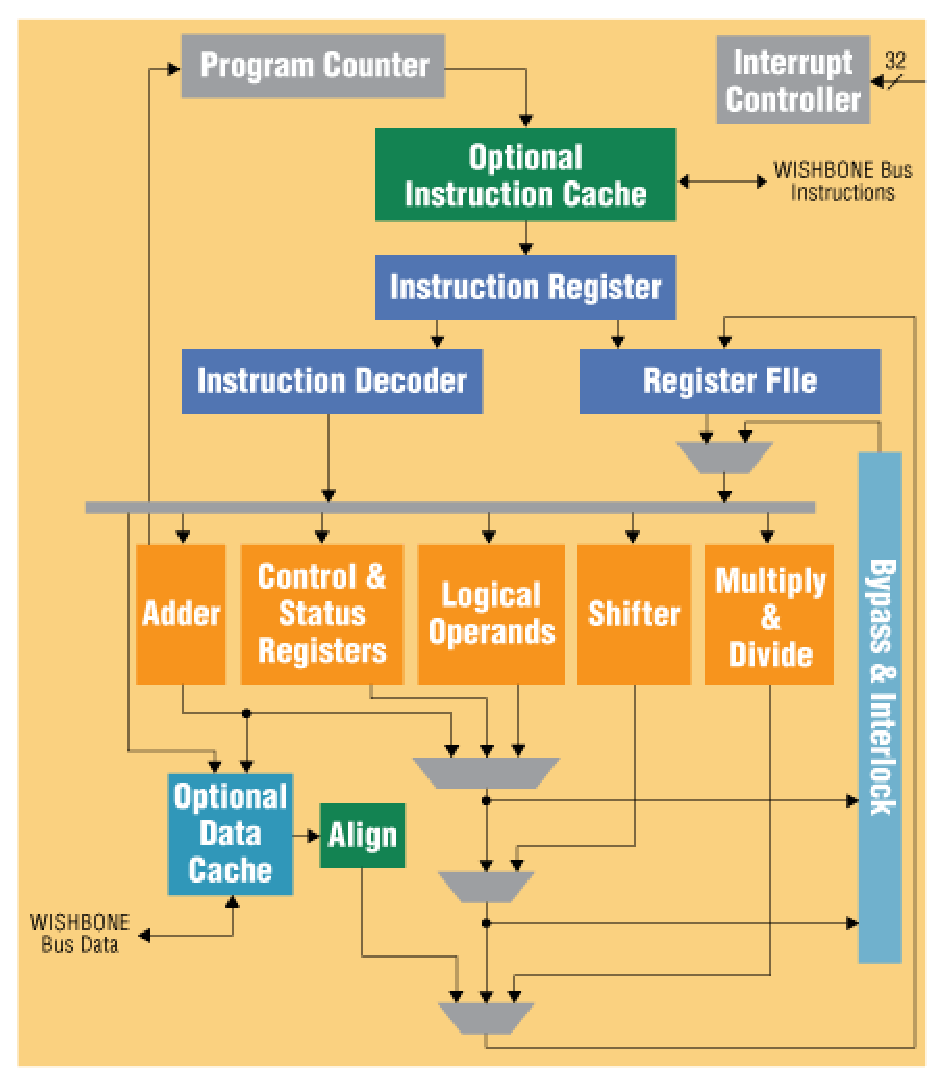
\includegraphics[height=90mm]{lm32arch.eps}
\caption{LatticeMico32 architecture (Lattice Semiconductor).}
\label{fig:lm32arch}
\end{figure}

The Milkymist system-on-chip uses LatticeMico32 with 2-way caches of 16KB each, and all the optional features enabled.

At the time this thesis is written, LatticeMico32 is the only hardware component that I have not developed specifically for the Milkymist project.

\section{Capabilities}
Linux has been ported to the Milkymist SoC (figure~\ref{fig:linux}). Since this is a community effort with a significant contribution by Takeshi Matsuya from Keio University, the details are not covered in this master thesis. Still, this demonstrates the ability of the platform to run complex software.

\begin{figure}[htp]
\centering
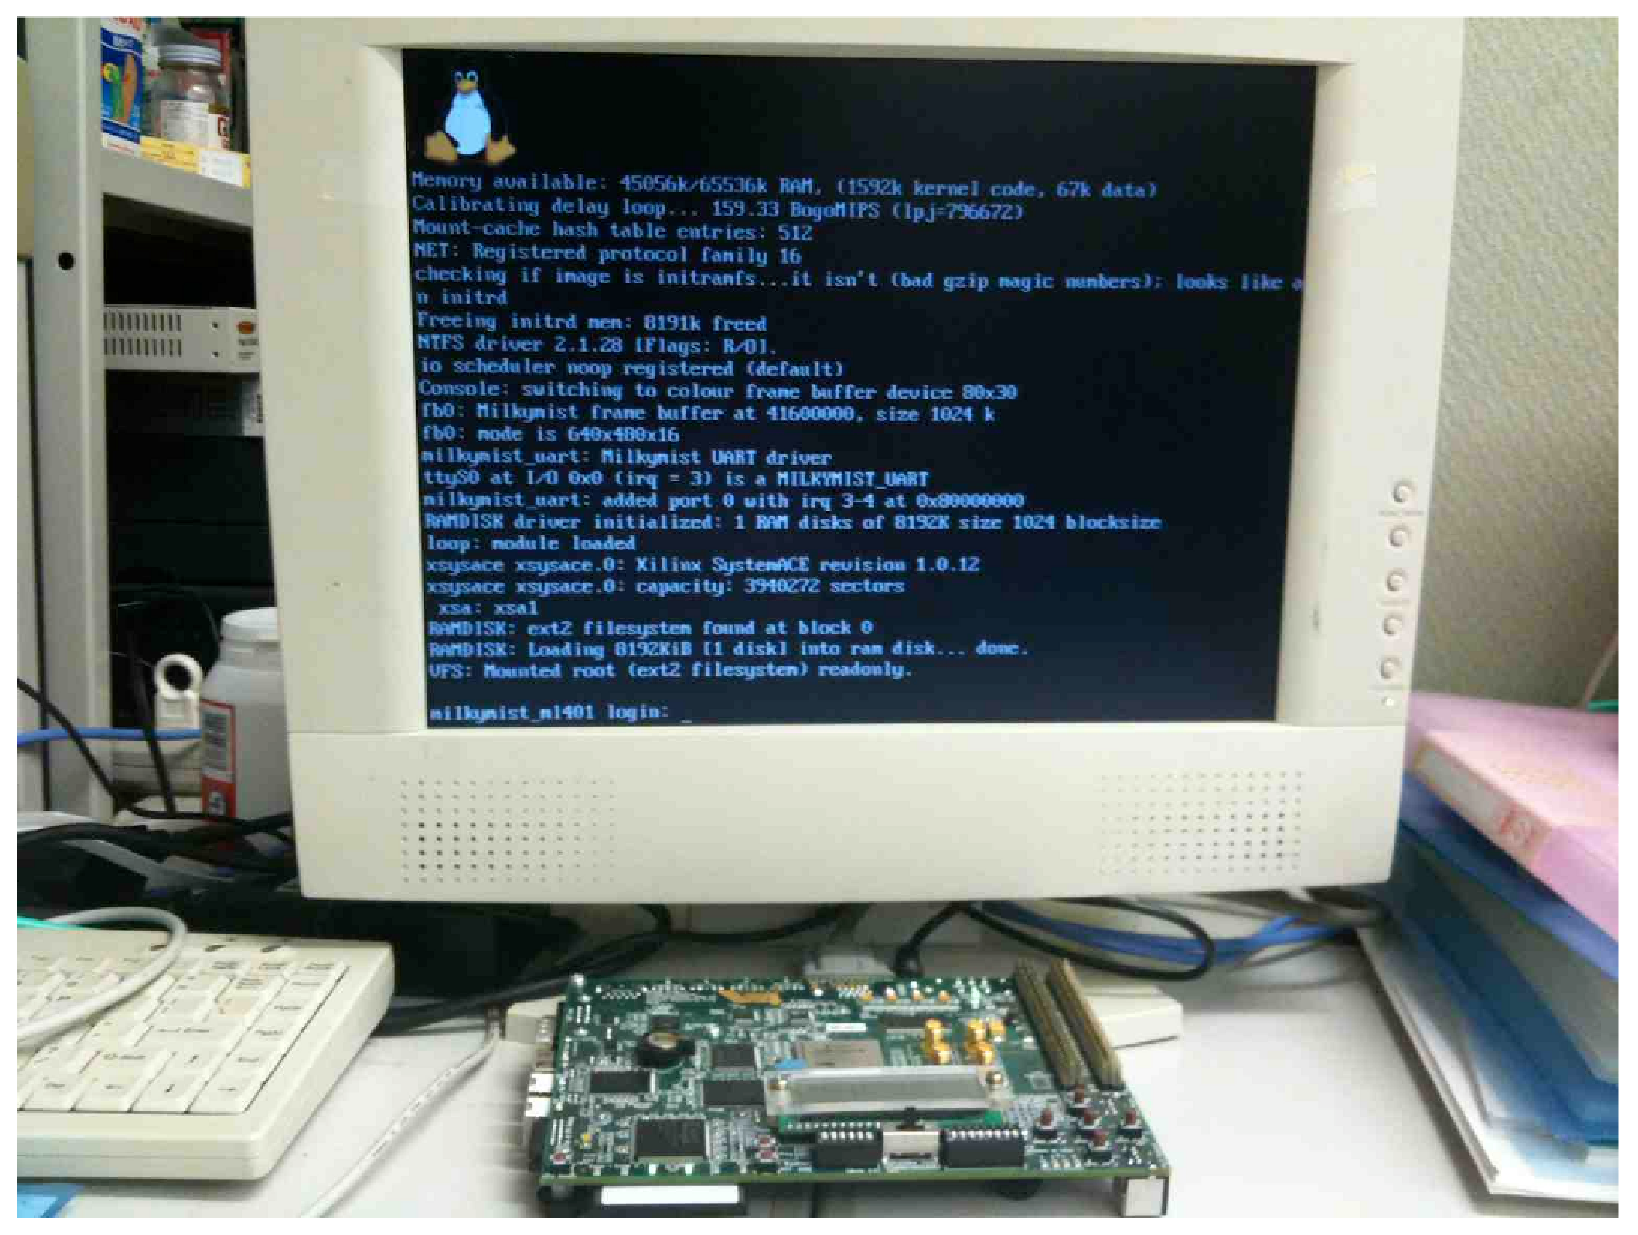
\includegraphics[height=100mm]{linux.eps}
\caption{Linux booting on the Milkymist SoC.}
\label{fig:linux}
\end{figure}

\section{Benchmarking}
The performance of the Milkymist SoC was compared to Microblaze~\cite{microblaze}, the proprietary Xilinx softcore SoC platform.

The benchmark used was the ``consumer'' MiBench~\cite{mibench} suite. By contrast to traditional benchmarks such as SPEC, MiBench is tailored to typical workloads of embedded systems. Only two benchmarks are missing from the ``consumer'' set: \verb!tiff2rgba! (it tried to use too much contiguous memory for the nommu Milkymist/Linux allocator to handle) and \verb!lame! (it crashed on Microblaze).

All tests were run on a Xilinx ML401 (XC4VLX25 FPGA) development board, with a system frequency of 100MHz.

For Milkymist, the configuration used was the default one of the port to the ML401 board:
\begin{itemize}
\item Processor with hardware multiplier, divider and barrel shifter
\item 16KB L1 instruction and data (write-through) cache (2-way set-associative)
\item No memory management unit (LatticeMico32 does not have one)
\item 16KB FML bridge write-back L2 cache (direct mapped)
\item HPDMC DDR SDRAM controller, 32-bit SDRAM bus width
\item 100MHz DDR SDRAM clock
\item Video output running at standard VGA resolution, consuming approximately 300MBps of memory bandwidth
\item Software: GCC 4.2.1 and Linux 2.6.23.
\end{itemize}

For Microblaze, the configuration is as follows:
\begin{itemize}
\item Processor with hardware multiplier, divider and barrel shifter
\item 16KB L1 instruction and data (write-through) cache (direct mapped, multi-way caches are not supported)
\item Full memory management unit
\item No L2 cache (not supported)
\item MPMC DDR SDRAM controller, 32-bit SDRAM bus width
\item 100MHz DDR SDRAM clock
\item No video output
\item Software: GCC 4.1.2 and Linux 2.6.32.4.
\end{itemize}

The comparison seems clearly in favor of Milkymist, with a rough 15\%-35\% (depending on the benchmark) reduction in execution time. Details are shown in figure~\ref{fig:mmvsmb} and in tables \ref{tab:milkymistspeed} and \ref{tab:microblazespeed}. Deviation is computed as:
\begin{equation}
\frac{|t_{1}-t_{2}|}{min(t_{1}, t_{2})}
\end{equation}
It is meant to check that the results are deterministic and reproducible.

\begin{figure}[htp]
\centering
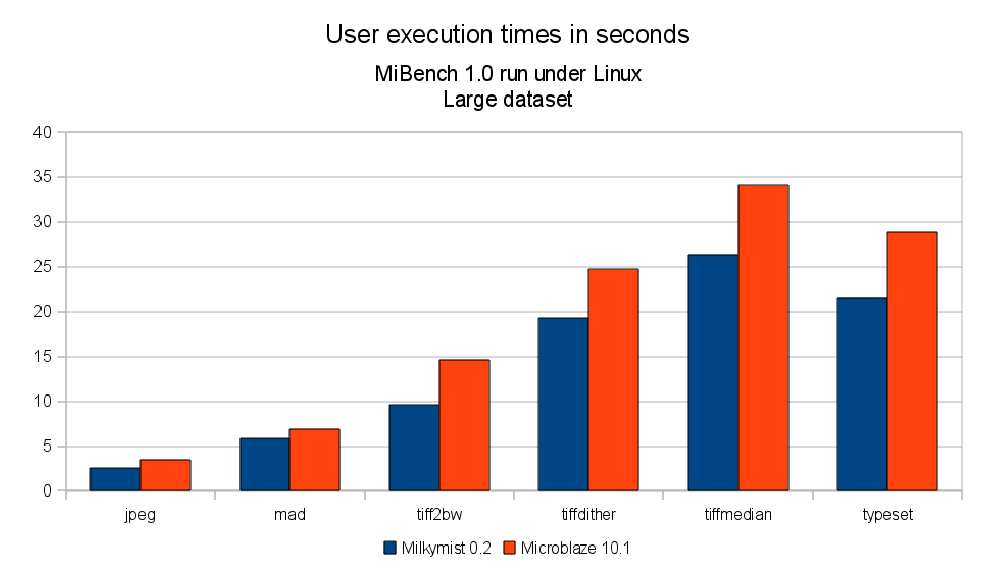
\includegraphics[height=75mm]{mm_vs_mb.eps}
\caption{Comparative MiBench results of Milkymist and Microblaze.}
\label{fig:mmvsmb}
\end{figure}

\begin{table}
\centering
\begin{tabular}{|l|l|l|l|l|}
\hline
\textbf{Benchmark} & \textbf{Run 1} & \textbf{Run 2} & \textbf{Average} & \textbf{Deviation}  \\
\hline
jpeg & 2.57 s & 2.54 s & 2.56 s & 1.18 \% \\
\hline
mad & 5.84 s & 5.87 s & 5.86 s & 0.51 \% \\
\hline
tiff2bw & 9.51 s & 9.69 s & 9.6 s & 1.89 \% \\
\hline
tiffdither & 19.28 s & 19.3 s & 19.29 s & 0.10 \% \\
\hline
tiffmedian & 26.48 s & 26.26 s & 26.37 s & 0.84 \% \\
\hline
typeset & 21.44 s & 21.79 s & 21.62 s & 1.63 \% \\
\hline
\end{tabular}
\label{tab:milkymistspeed}
\caption{User execution times on Milkymist 0.2.}
\end{table}

\begin{table}
\centering
\begin{tabular}{|l|l|l|l|l|}
\hline
\textbf{Benchmark} & \textbf{Run 1} & \textbf{Run 2} & \textbf{Average} & \textbf{Deviation}  \\
\hline
jpeg & 3.42 s & 3.58 s & 3.5 s & 4.68 \% \\
\hline
mad & 6.72 s & 7.11 s & 6.92 s & 5.80 \% \\
\hline
tiff2bw & 15.19 s & 14.12 s & 14.66 s & 7.58 \% \\
\hline
tiffdither & 24.72 s & 24.68 s & 24.7 s & 0.16 \% \\
\hline
tiffmedian & 35.02 s & 33.05 s & 34.04 s & 5.96 \% \\
\hline
typeset & 28.91 s & 28.83 s & 28.87 s & 0.28 \% \\
\hline
\end{tabular}
\label{tab:microblazespeed}
\caption{User execution times on Microblaze 10.1.}
\end{table}


The root causes of this performance improvement were not investigated; but since LatticeMico32 and Microblaze share a very close architecture, it is suspected that these differences are vastly explained by the combination of the low-latency HPDMC controller and the improved caches.

The main point of this comparison is to confirm the viability of Milkymist as a powerful SoC platform, that can withstand the competition with proprietary solutions.

\chapter{Texture mapping unit}
\label{ch:tmu}

\chapter{Floating point coprocessor}

\bibliography{thesis}{}
\bibliographystyle{plain}

\end{document}
